\documentclass[a4paper, 12pt]{article}
\usepackage{cmap}
\usepackage{amssymb}
\usepackage{amsmath}
\usepackage{graphicx}
\usepackage{amsthm}
\usepackage{upgreek}
\usepackage{setspace}
\usepackage{color}
\usepackage[T2A]{fontenc}
\usepackage[utf8]{inputenc}
\usepackage[normalem]{ulem}
\usepackage{mathtext} % русские буквы в формулах
\usepackage[left=2cm,right=2cm, top=2cm,bottom=2cm,bindingoffset=0cm]{geometry}
\usepackage[english,russian]{babel}
\usepackage[unicode]{hyperref}
\newenvironment{Proof} % имя окружения
{\par\noindent{$\blacklozenge$}} % команды для \begin
{\hfill$\scriptstyle\boxtimes$}
\newcommand{\Rm}{\mathbb{R}}
\newcommand{\Cm}{\mathbb{C}}
\newcommand{\Z}{\mathbb{Z}}
\newcommand{\I}{\mathbb{I}}
\newcommand{\N}{\mathbb{N}}
\newcommand{\rank}{\operatorname{rank}}
\newcommand{\Ra}{\Rightarrow}
\newcommand{\ra}{\rightarrow}
\newcommand{\FI}{\Phi}
\newcommand{\Sp}{\text{Sp}}
\renewcommand{\leq}{\leqslant}
\renewcommand{\geq}{\geqslant}
\renewcommand{\alpha}{\upalpha}
\renewcommand{\beta}{\upbeta}
\renewcommand{\gamma}{\upgamma}
\renewcommand{\delta}{\updelta}
\renewcommand{\varphi}{\upvarphi}
\renewcommand{\phi}{\upvarphi}
\renewcommand{\tau}{\uptau}
\renewcommand{\lambda}{\uplambda}
\renewcommand{\psi}{\uppsi}
\renewcommand{\mu}{\upmu}
\renewcommand{\omega}{\upomega}
\renewcommand{\d}{\partial}
\renewcommand{\xi}{\upxi}
\renewcommand{\epsilon}{\upvarepsilon}
\newcommand{\intx}{\int\limits_{x_0}^x}
\newcommand\Norm[1]{\left\| #1 \right\|}
\newcommand{\sumk}{\sum\limits_{k=0}^\infty}
\newcommand{\sumi}{\sum\limits_{i=0}^\infty}
\newtheorem*{theorem}{Теорема}
\newtheorem*{cor}{Следствие}
\newtheorem*{lem}{Лемма}
\begin{document}
	\section*{Метод Лобачевского для отыскания корней многочлена}
	\subsubsection*{Условие}
	Вычислить с точностью $\epsilon=10^{-1}$ корни алгебраического уравнения $$x^3-2x^2+3x +10 = 0.$$
	\subsubsection*{Алгоритм решения}
	Для решения задачи методом Лобачевского нам понадобятся следующие формулы:
\begin{enumerate}
	\item соотношения для коэффициентов: 
	\begin{eqnarray}
		\begin{cases}
			a_0^{(1)} = a_0^2,\\
			a_1^{(1)} =2a_0a_2 - a_1^2,\\
			a_2^{(1)} = 2a_0a_4 - 2a_1a_3 + a_2^2,\\
			\dotfill\\
			a_n^{(1)} = (-1)^na_n^2
		\end{cases}
	\end{eqnarray}
	(конкретно эта формула позволяет перейти от итерации 0 к итерации 1, но для перехода от $k$ к $k+1$ соотношения такие же).\\\\
	Для нашего случая соотношения будут иметь вид
	\begin{eqnarray}
		\begin{cases}
			a_0^{(1)} = a_0^2,\\
			a_1^{(1)} =2a_0a_2 - a_1^2,\\
			a_2^{(1)} = - 2a_1a_3 + a_2^2,\\
			a_3^{(1)} = -a_3^2
		\end{cases}
	\end{eqnarray}
	\item формула для вычисления корней \begin{eqnarray}
		x_i\approx\sqrt[2^k]{ - \dfrac{a_i^{(k)}}{a_{i-1}^{(k)}}},\quad i =\overline{1,n}.
	\end{eqnarray}
\end{enumerate} 
\textbf{Замечание.} Метод Лобачевского после прохождения всего цикла возвращает значения корней \textit{по модулю}. Поэтому необходимо подстановкой в исходное уравнение проверить, с каким знаком нужно раскрывать модуль.\\\\
	Для решения методом Лобачевского удобно составить следующую таблицу (каждый столбец -- это коэффициенты, а в конце значения корней на каждой итерации в порядке убывания):
	$$
	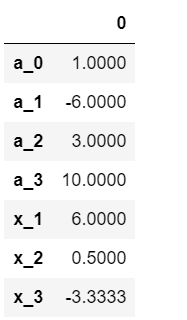
\includegraphics[scale=0.6]{img05}
	$$
	где мы посчитали по формулам (3) $$x_1 = - \dfrac{a_1}{a_0},\quad x_2 = - \dfrac{a_2}{a_1}, \quad x_3 = - \dfrac{a_3}{a_2}.$$
	Считаем коэффициенты и корни из соотношений (2) $$\begin{cases}
		a_0^{(1)} = a_0^2 = 1,\\
		a_1^{(1)} =2a_0a_2 - a_1^2 = -30,\\
		a_2^{(1)} = - 2a_1a_3 + a_2^2 = 129,\\
		a_3^{(1)} = -a_3^2 = -100
	\end{cases}$$
	По формулам (3)
	$$x_1^{(1)} = \sqrt{- \dfrac{a_1^{(1)}}{a_0^{(1)}}} \approx 5.4772,\quad x_2^{(1)} = \sqrt{- \dfrac{a_2^{(1)}}{a_1^{(1)}}} \approx 2.0736,\quad x_3^{(1)} = \sqrt{- \dfrac{a_3^{(1)}}{a_2^{(1)}}} \approx 0.8805.$$
	$$
	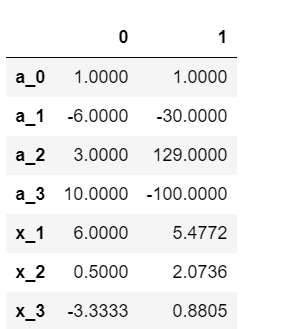
\includegraphics[scale=0.6]{img06}
	$$
	Вычислим погрешность. Лучше всего считать разницу для каждого корня, чтобы быть уверенными в том, что каждый корень достиг нужной точности:
	$$|x_1^{(1)} - x_1^{(0)}| = 0.228 > 10^{-1},\quad|x_2^{(1)} - x_2^{(0)}| = 1.574 > 10^{-1},\quad |x_3^{(1)} - x_3^{(0)}| = 4.214 > 10^{-1}.$$
	Далее проделываем все то же самое, аналогично случаю отыскания одного корня. Тогда в конечном итоге получается таблица вида:
	$$
	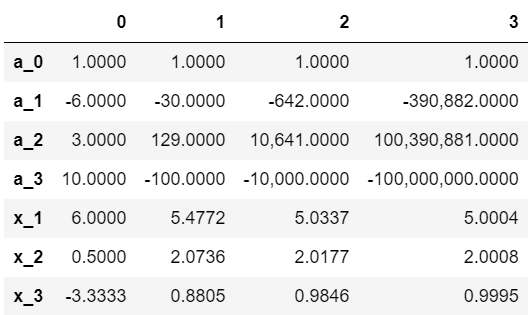
\includegraphics[scale=0.6]{img07}
	$$
	Таким образом, округлив, получим значения $$x_1 \approx 5,\quad x_2 \approx 2,\quad x_3 \approx 1.$$
	Но это абсолютные значения истинных корней. Далее непосредственной подстановкой необходимо выбрать, какие из значений $x=\{-5, -2, -1, 1, 2, 5\}$ действительно являются корнями исходного уравнения.\\\\
	В данном случае подходят значения $$x=\{1,2,5\}.$$
\end{document}